%% LaTeX-Beamer template for KIT design
%% by Erik Burger, Christian Hammer
%% title picture by Klaus Krogmann
%%
%% version 2.1
%%
%% mostly compatible to KIT corporate design v2.0
%% http://intranet.kit.edu/gestaltungsrichtlinien.php
%%
%% Problems, bugs and comments to
%% burger@kit.edu

\documentclass[18pt]{beamer}
%% SLIDE FORMAT
\usepackage[utf8]{inputenc}
% use 'beamerthemekit' for standard 4:3 ratio
% for widescreen slides (16:9), use 'beamerthemekitwide'

%\usepackage{templates/beamerthemekit}
\usepackage{wrapfig}
\usepackage{hyperref}
\usepackage{algpseudocode}
 \newcommand{\real}{\mathbb{R}}
 \newcommand{\nat}{\mathbb{N}}
 \newcommand{\Oh}{\mathcal{O}}
 \newcommand{\oh}{\mathrm{o}}
 \newcommand{\SP}{\mathrm{SP}}

% \usepackage{templates/beamerthemekitwide}

%\usepackage{epigraph}

% for quotes

\AtBeginSection[] % Do nothing for \section*
{
\begin{frame}<beamer>
\frametitle{Gliederung}
\tableofcontents[currentsection]
\end{frame}
}


\usepackage{biolinum}

%% TikZ INTEGRATION

% use these packages for PCM symbols and UML classes
% \usepackage{templates/tikzkit}
% \usepackage{templates/tikzuml}

% the presentation starts here

\title[Algo I Tut]{2. Algorithmen Tutorium I}
\subtitle{Rechnen im O-Kalkül}
\author[Zangerle]{Konstantin Zangerle}

\institute{Institut für Theoretische Informatik}

\usepackage{listings}
\usepackage{color}

\definecolor{mygreen}{rgb}{0,0.6,0}
\definecolor{mygray}{rgb}{0.5,0.5,0.5}
\definecolor{mymauve}{rgb}{0.58,0,0.82}

\lstset{ %
  backgroundcolor=\color{white},   % choose the background color
  basicstyle=\footnotesize,        % size of fonts used for the code
  breaklines=true,                 % automatic line breaking only at whitespace
  captionpos=b,                    % sets the caption-position to bottom
  commentstyle=\color{mygreen},    % comment style
  escapeinside={\%*}{*)},          % if you want to add LaTeX within your code
  keywordstyle=\color{blue},       % keyword style
  stringstyle=\color{mymauve},     % string literal style
}

% Bibliography

\begin{document}

% change the following line to "ngerman" for German style date and logos
%\selectlanguage{ngerman}

%title page
\begin{frame}
\titlepage
\end{frame}

%table of contents
\begin{frame}{Gliederung}
 \tableofcontents
\end{frame}

\section{Besprechung der Übungsaufgaben}
\begin{frame}{Besprechung der Übungsaufgaben}
Häufige Fehler
\begin{itemize}
 \item return beendet automatisch eine Funktion
 \item Aufgabe 2: Basis beachten
\end{itemize}

\end{frame}

\section{O Kalkül}
\begin{frame}{Limes Definitionen O-Kalkül}
 $f \in \Oh(g) \iff \limsup_{x \to \infty}| \frac{f(x)}{g(x)}| < \infty$ \\
 $f \in \Theta(g) \iff 0 < \liminf_{x \to \infty} | \frac{f(x)}{g(x)} |< \limsup_{x \to \infty} |\frac{f(x)}{g(x)} |< \infty$ \\
 $f \in \Omega(g) \iff \liminf_{x \to \infty} \frac{f(x)}{g(x)} > 0$ \\
\end{frame}

\begin{frame}{Aussagen im O Kalkül}
Beweist/widerlegt verschiedene Aussagen im O-Kalkül.
  \begin{itemize}
    \item $f(n) + g(n) = \Oh({\max(f(n),g(n))})$
    \item Auf der Menge der asymptotisch positiven Funktionen ist 
      $$f \sim_{\Theta} g \quad:\Longleftrightarrow\quad f \in \Theta(g)$$
      eine Äquivalenzrelation.
    \item $2^{n} = \Oh({3^n})$
    \item $[ f(n) + g(n) ]^2 = \Oh{f(n)^2} + \Oh{g(n)^2}$
    \item $\sqrt{n} = \Oh({{\log n}})$
    \item $n^2(1+\sqrt{n}) = \Oh({n^2 \log n})$
    \item $3n^2 + \sqrt{n} = \Oh({n^2})$
    \item $n^2 = \Oh({2^n})$
    \item $2^{2n} = \Oh({2^n})$
  \end{itemize}
\end{frame}

\begin{frame}{O Kalkül}
  \begin{itemize}
    \item Für jedes der folgenden Paare von Funktionen gilt entweder $f(n) = \Oh (g(n))$, $f(n) = \Omega(g(n))$ oder $f(n) = \Theta(g(n))$. Geben Sie an, welche Beziehung gilt und beweisen Sie deren Gültigkeit:
    \begin{enumerate}
      \item  $f(n) = \log n^2$; $g(n)= \log n + 5$
      \item  $f(n) = \sqrt{n}$; $g(n)= \log n^2$
      \item  $f(n) = n \log n + n$; $g(n)= \log n$
      \item  $f(n) = n$; $g(n)= \log^2 n$
    \end{enumerate}
    \item Für jedes der folgenden Paare von Funktionen gilt entweder $f(n) = \Oh(g(n))$, $g(n) = \Omega(f(n))$ oder beides. Geben Sie an, welche Beziehung gilt und beweisen Sie deren Gültigkeit:
    \begin{enumerate}
      \item  $f(n) = 4n \log n +n$; $g(n)= (n^2 -n) / 2$
      \item  $f(n) = n + \log n$; $g(n)= \sqrt{n}$
      \item  $f(n) = (n^2 -n)/2$; $g(n)= 6n$
    \end{enumerate}
  \end{itemize}
\end{frame}


\section{Mergin Problem}
\begin{frame}[fragile]{Mergin Problem}
Das Merging-Problem ist folgendermaßen definiert:\\
\textbf{Gegeben:} zwei aufsteigend sortierte Arrays $A[1..n_1], B[1..n_2]$ von natürlichen Zahlen\\
\textbf{Gesucht:} das aufsteigend sortierte Array $C[1..(n_1+n_2)=:n]$ von natürlichen Zahlen, das genau die Zahlen von $A$ und $B$ enthält\\



Beweisen Sie die Korrektheit des vorgegebenen Algorithmus, in dem Sie die vorgebenen Invarianten 
und Assertions beweisen. Beweisen Sie außerdem, dass der vorgegebene Algorithmus linearen 
Zeitverbrauch hat.

\end{frame}
\begin{frame}[fragile]
\footnotesize % nötig für eine Folie
  \begin{algorithmic}[1]
      \Function{merge}{$A : $ Array $[1..n_1]$ of $\nat_{\geq 0} $, $B : $ Array $[1..n_2]$ of $\nat_{\geq 0} $}
	\Require{$A[i] \leq A[j]$ \quad $ \forall i \leq j$ mit  $i, j \in \{1,..., n_1\}$}
	\Require{$B[i] \leq B[j]$ \quad $ \forall i \leq j$ mit $i, j \in \{1,..., n_2\}$}
	\State $A[n_1+1] := \infty$, $B[n_2+1] := \infty$
	\State $n := n_1 + n_2$ 
	\State $j_A := 1$, $j_B := 1$;
	\For{$i:=1$ to $n$}
		  \State  $C[i] = \min(A[j_A],B[j_B])$
		  \If{ $A[j_A] < B[j_B]$}
		    \State $j_A = j_A + 1$ 
		  \Else
		    \State $j_B = j_B + 1$ 
		  \EndIf
	  \State \textbf{invariant }$C[1..i]$ enthält genau $A[1..j_A-1], B[1..j_B-1]$ 
	  \State \textbf{invariant }$\forall k \in \{1..j_B-1\}: B[k] \leq A[j_A] $; $\forall k \in \{1..j_A-1\}: A[k] \leq B[j_B] $ 
	  \State \textbf{invariant }$C[1..i]$ ist sortiert 
        \EndFor
        \State \textbf{assert} $j_A = n_1+1, j_B = n_2 + 1$ 
        \State \textbf{postcondition}  $C[i] \leq C[j]$ \quad $ \forall i \leq j,$ $i, j \in \{1,..., n\}$
        \State \textbf{postcondition} $C[1..n]$ enthält genau $A[1..n_1], B[1..n_2]$ 
      \State \Return C
      \EndFunction
    \end{algorithmic}
\end{frame}
\begin{frame}{Musterlösung - Laufzeit}
\textbf{Laufzeit: } Jeder Aufruf der Schleife benötigt konstant viel Zeit. Da die Schleife von $1$ bis $n$ läuft ist daher die Laufzeit offensichtlich $\Theta(n)$.\\ 
\end{frame}

\begin{frame}{Musterlösung - Korrektheit (Z. 12)}
\begin{itemize}
 \item Induktionsanfang $i=1$: Es wird genau eins der Arrays ausgewählt. Danach wird vom ausgewählten Array der Pointer um eins erhöht. D.h. im Fall $A[j_A] < B[j_B]$ wird $j_A$ zu 2 und $j_B$ bleibt 1. Dann gilt Behauptung. Der andere Fall geht analog.
 \item Induktionsvoraussetzung: $C[1..i-1]$ enthält genau $A[1..j_A-1], B[1..j_B-1]$ 
 \item 	Induktionsschluss $i-1 \rightsquigarrow i$: Im Fall $A[j_A] < B[j_B]$ wurde $A[j_A]$ hinzugefügt und $j_A$ wurde um eins erhört. Also gilt die Behauptung. Der andere Fall gilt analog.
\end{itemize}	
\end{frame}

\begin{frame}{Musterlösung - Korrektheit (Z. 13)}
\begin{itemize}
 \item Induktionsanfang $i=1$: zu dem Zeitpunkt befindet sich nur ein Elementi $C[1]$ im Array $C$. Wegen Zeile 8 ist $C[1] = \min(A[1],B[1])$. Im Fall $C[1] = A[1]$ wird $j_A$ um eins erhöht und es gilt offensichtlich $A[1] \leq B[1]$. Die Behauptung gilt also. Der andere Fall geht analog.
 \item Induktionsvoraussetzung: Die Invariante ist zum Zeitpunkt $i-1$ erfüllt. D.h. $B[k] \leq A[j_A] \quad  \forall k \in \{1..j_B-1\}$, $A[k] \leq B[j_B]\quad  \forall k \in \{1..j_A-1\}$
 \item Induktionsschluss $i-1 \rightsquigarrow i$: Wir betrachten den Fall, dass in Zeile 8 $C[i] =  A[j_A]$ gewählt wird. In diesem Fall ist $j_{A_{\text{neu}}} = j_{A_{\text{alt}}} +1 $ und $A[j_{A_{\text{alt}}}] \leq B[j_{B_{\text{alt}}}]$. Umstellen liefert  $A[j_{A_{\text{neu}}}-1] \leq B[j_{B_{\text{alt}}}]$.
	Insbesondere impliziert das zusammen mit der Induktionsvoraussetzung die Behauptung $A[k] \leq B[j_{B_\text{alt}}]\quad  \forall k \in \{1..j_{A_{\text{neu}}}-1\}$. Der andere Fall geht analog.  
\end{itemize}

	
        
	
\end{frame}
\begin{frame}{Invariante in  Zeile 14}
\begin{itemize}
 \item Induktionsanfang $i=1$: zu dem Zeitpunkt befindet sich nur ein Element im Array $C$. Also ist $C$ sortiert. \\
 \item Induktionsvoraussetzung: Die Invariante ist zum Zeitpunkt $i-1$ erfüllt. D.h. $C[1..i-1]$ ist sortiert.\\
 \item 	Induktionsschluss $i-1 \rightsquigarrow i$: Da die beiden Arrays $A, B$ aufsteigend sortiert sind, ist $A[k] \leq A[j_A] \quad \forall k \leq  j_A$ und $B[k] \leq B[j_B] \quad \forall k \leq j_B$. Mit den vorherigen Invarianten folgt dann, $C[k] \leq A[j_A], C[k] \leq B[j_B] \quad 	\forall k \leq i-1$. Also folgt insbesondere $C[k] \leq C[i] = \min(A[j_A],B[j_B]) \quad \forall k \leq i-1 $. Also ist $C[1..i]$ aufsteigend sortiert.

\end{itemize}
\end{frame}

\begin{frame}{Assertion in Zeile 16:} 
Nach Ausführung der Schleife wurde $j_A$ $n_1$ mal erhöht und $j_B$ wurde $n_2$ mal erhört. Da beide werde mit 1 initialisiert wurden gilt die Behauptung.  

Insgesamt folgt nach Ausführung der Schleife:  $C[1..n]$ enthält genau $A[1..n_1]$ und $B[1..n_2]$ sowie $C[1..n]$ ist sortiert. Unser Algorithmus arbeitet also korrekt.
 
\end{frame}


\begin{frame}
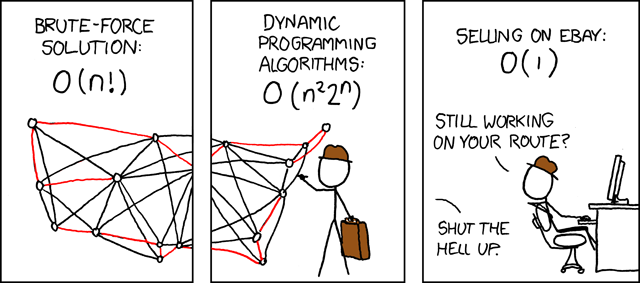
\includegraphics[scale=0.5]{travelling_salesman_problem} \\
License: http://creativecommons.org/licenses/by-nc/2.5/ \\
by xkcd.com/399
\end{frame}

\end{document}
